
\let\textcircled=\pgftextcircled
\chapter{System design}

\initial{A}s mentioned in Section \ref{sec:methodology}, the design of the Obstacle Collision Avoidance System will follow the Systems Engineering approach.
The main reason is that Systems Engineering provides some methods that prevent the errors with the highest consequences when the system to be designed is complex.
As explained by Rolls-Royce Global Chief of Systems Engineering \cite{beasley2015}:
\begin{quote}
	\itshape
	Systems Engineering collects and organises all the information needed to understand the whole problem, explores it from all angles, and then finds the most appropriate system solution.
\end{quote}

Furthermore, A key study published through INCOSE \cite{incoseuk2016} looked at the phase of detection of errors, and the consequent cost of fixing them.
Cost modelling was validated against a cross-industry range of defence and aerospace projects.
Figure \ref{fig:incose} shows the results of the study.

\begin{figure}[htbp]
	\centering
	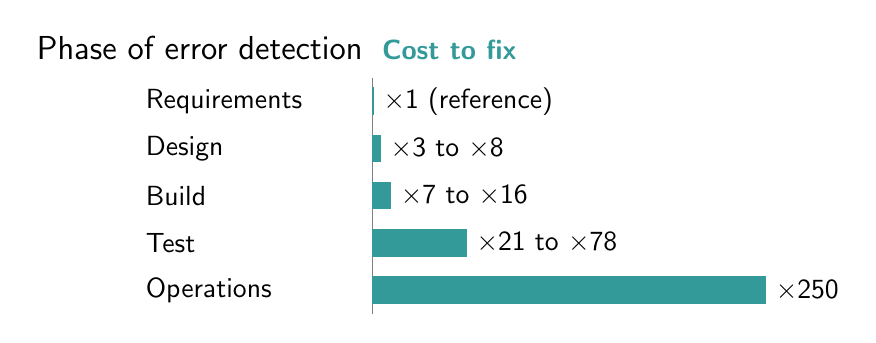
\begin{tikzpicture}

		\colorlet{blueish}{teal!80}

		%\draw[step=1cm,gray,very thin] (0,0) grid (9,6);

		\node[above left,black] at (3,6.2) {\sffamily \large Phase of error detection};
		\node[above right,blueish] at (3,6.2) {\sffamily \bfseries Cost to fix};
		\draw[black!50] (3,6.1) -- (3,3.1);
		\draw[blueish, line width=0.35cm] (3,5.8) -- (3.02,5.8);
			\node[right] at (0,5.8) {\sffamily Requirements};
			\node[right] at (3.02,5.8) {\sffamily $\times$1 (reference)};
		\draw[blueish, line width=0.35cm] (3,5.2) -- (3.11,5.2);
			\node[right] at (0,5.2) {\sffamily Design};
			\node[right] at (3.11,5.2) {\sffamily $\times$3 to $\times$8};
		\draw[blueish, line width=0.35cm] (3,4.6) -- (3.24,4.6);
			\node[right] at (0,4.6) {\sffamily Build};
			\node[right] at (3.24,4.6) {\sffamily $\times$7 to $\times$16};
		\draw[blueish, line width=0.35cm] (3,4) -- (4.2,4);
			\node[right] at (0,4) {\sffamily Test};
			\node[right] at (4.2,4) {\sffamily $\times$21 to $\times$78};
		\draw[blueish, line width=0.35cm] (3,3.4) -- (8,3.4);
			\node[right] at (0,3.4) {\sffamily Operations};
			\node[right] at (8,3.4) {\sffamily $\times$250};

	\end{tikzpicture}
	\caption{Cost to fix a design error. {\footnotesize Source: \cite{incoseuk2016}}}
	\label{fig:incose}
\end{figure}


Hence, in the present chapter, some of the most relevant Systems Engineering tools from the NASA Systems Engineering Handbook \cite{nationalaeronauticsandspaceadministration2007} will be applied


\section{Requirements capture}

